\subparagraph{lab 1 \& 2}
The LED on the board blinked successfully and followed the rule we set in the programs.
\subparagraph{lab 3 \& 4}
The LED brick we connected to the board worked normally, and blinks as was programmed before.
\subparagraph{lab 5}
The LED brick is controlled by the button brick. When we press the button the LED turns on, and it turns off when we release the button.
\subparagraph{lab 6}
\begin{figure}
	\centering
	\label{fig:2}
	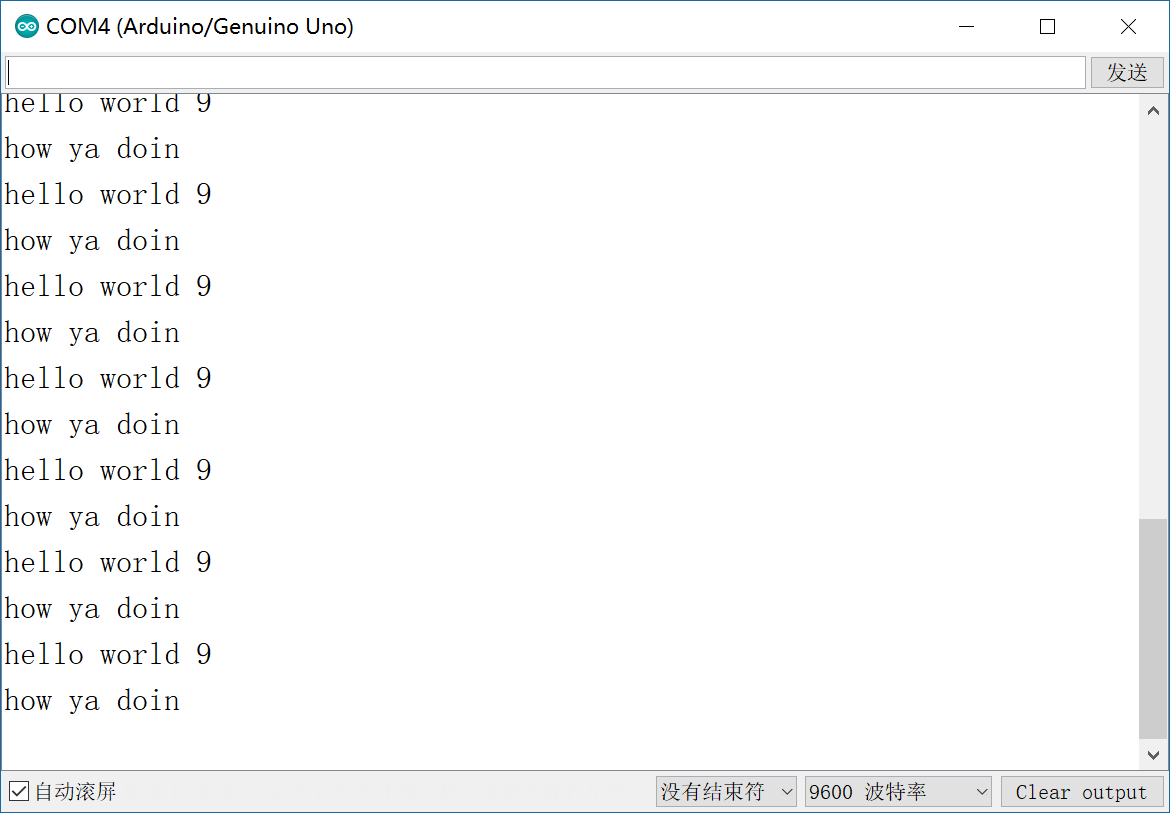
\includegraphics[width = \linewidth]{images/06_helloworld.PNG}
	\caption{result of lab 6}
\end{figure}
The messages that the processor sends(figure 2) show correctly on the serial display window. It keeps printing "hello world 9" and "how ya doin" to the screen, with every sentence displayed on one line.
\subparagraph{lab 7}
\begin{figure}
	\centering
	\label{fig:23}
	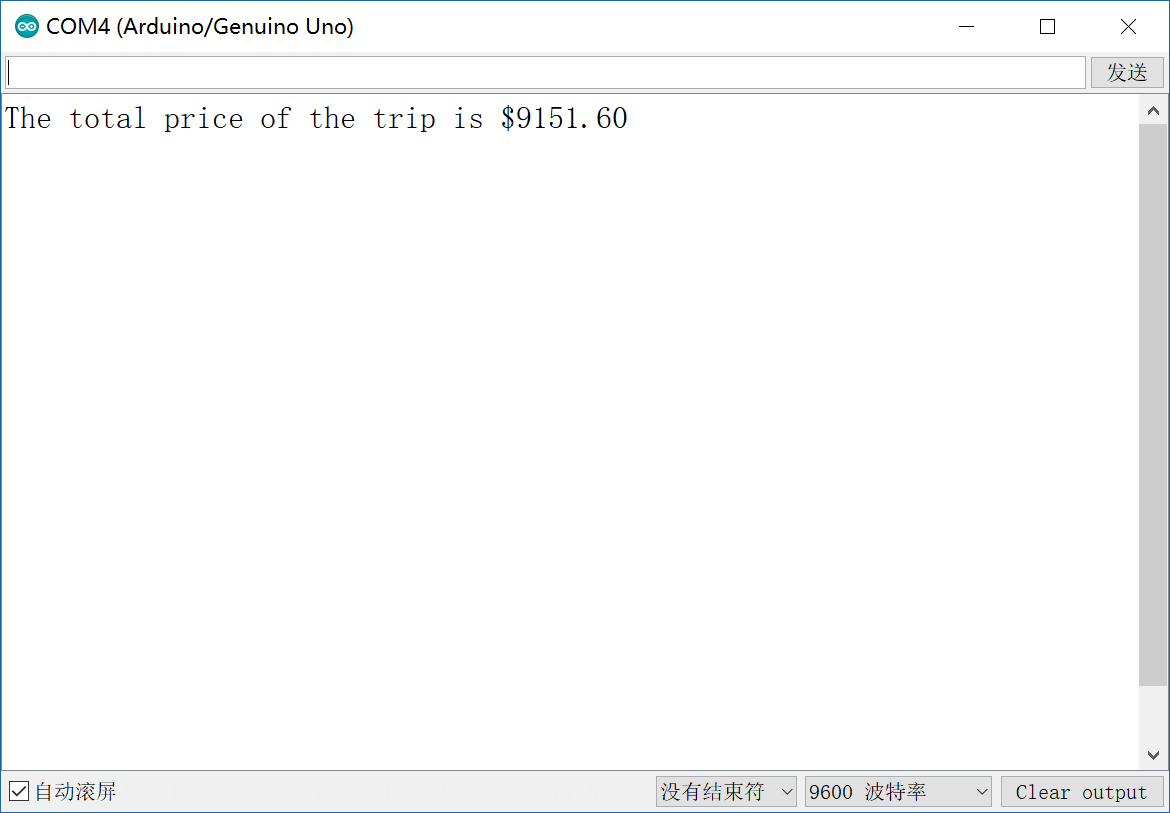
\includegraphics[width = \linewidth]{images/07_price.PNG}
	\caption{result of lab 7}
\end{figure}
The result of calculation is sent to the computer through the serial, and then displayed on the monitor screen correctly(figure 3).
\subparagraph{lab 8}
The names of the first two members are correctly shown on the first row of the display screen of the LCD connected to the microprocessor, and the name of the third member is correctly shown on the second row.
\subparagraph{lab 9}
The cursor on the screen of the LCD connected to the microprocessor can be incrementally moved by one space, left (by one button) or right(by another button). When the cursor meets the end of the first row, (if moved right), the cursor will move to the beginning of the second row. When the cursor meets the end of the second row,(if moved right), the cursor will move to the beginning of the second row.
\subparagraph{lab 10}
\begin{figure}
	\centering
	\label{fig:3}
	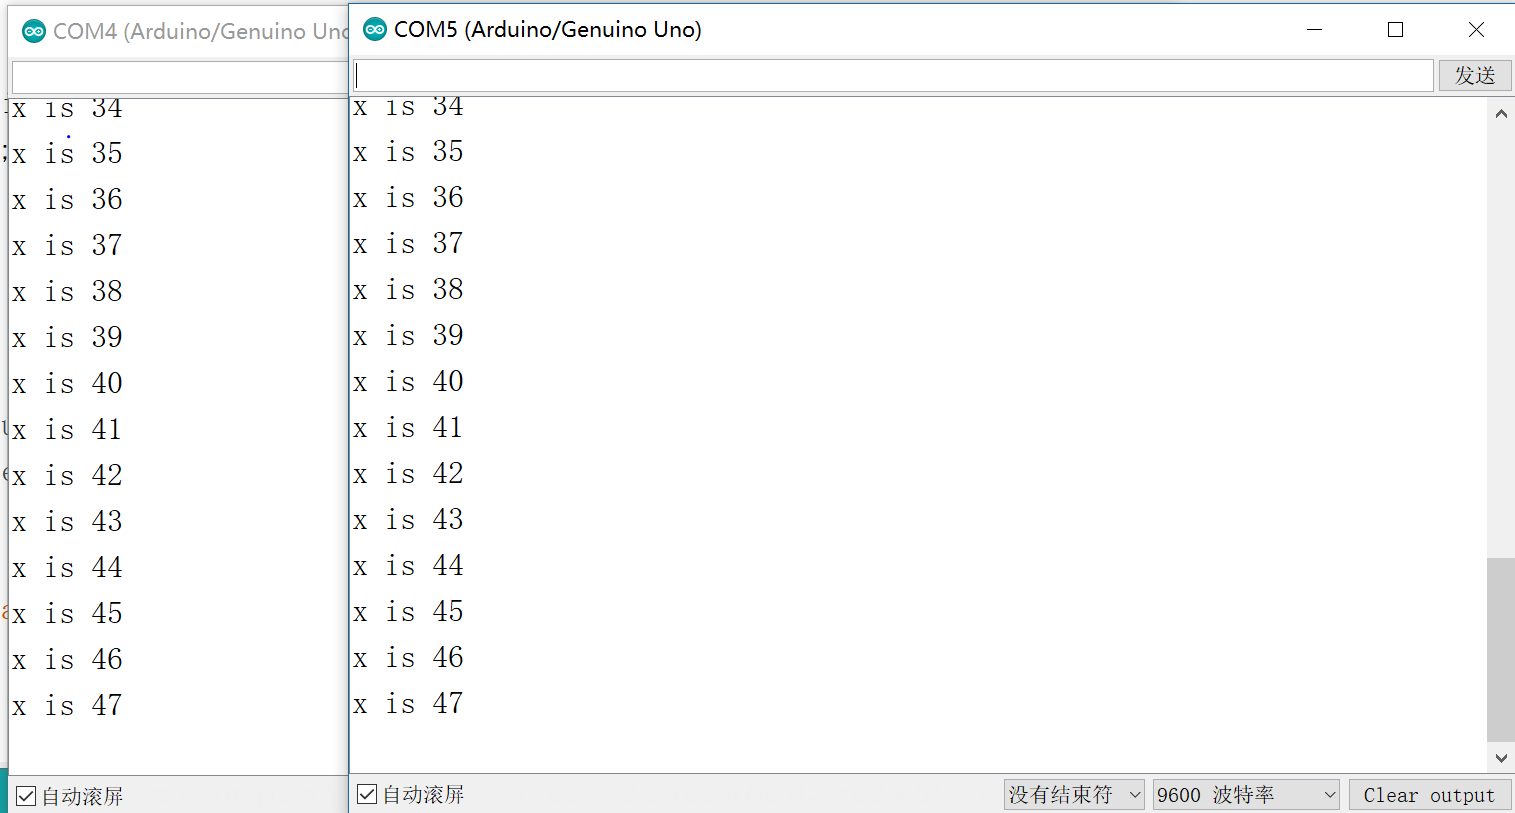
\includegraphics[width = \linewidth]{images/09_i2c.PNG}
	\caption{result of lab 10}
\end{figure}
The serial monitors of the two microprocessors on the PC displays the same text series(figure 4).
\subparagraph{lab 11}
The LED brick on slave can be turned ON and OFF by signals over I2C from a button brick on the master. When the button brick is pressed, the LED is turned On.